% -- coding: UTF-8 --
\documentclass[11pt,UTF8,oneside]{mybook}
\usepackage{xeCJK}
\usepackage{lipsum}
\usepackage{pythonhighlight}
\usepackage[colorlinks,linkcolor=black]{hyperref}
\usepackage{indentfirst}
\usepackage{url}
\usepackage{graphicx}
\usepackage[top=1in, bottom=1in, left=1.25in, right=1.25in]{geometry}
\usepackage{enumerate}
\usepackage{booktabs}
\usepackage{amsmath,amssymb}


\setCJKmainfont[BoldFont=FandolSong-Bold.otf,ItalicFont=FandolKai-Regular.otf]{FandolSong-Regular.otf}
\setCJKsansfont[BoldFont=FandolHei-Bold.otf]{FandolHei-Regular.otf}
\setCJKmonofont{FandolFang-Regular.otf}



\begin{document}
\setlength{\parindent}{2em} \title{Spider Book in Python} \author{华聪}
\date{} \setlength{\parskip}{5pt} \setlength{\baselineskip}{1.5em}

\maketitle
\frontmatter



\chapter{前言}

\beforecontent{总觉得自己不是一个会说话的人,偏偏自己又有很多话要说,那
  就写下来吧!}{华聪}

\section{更新说明}

由于时间有限,不可能一下就把整本书写完。所以,就放出这么一个栏目,每次
把更新的内容和时间都列出来。

\begin{table}[htb]
  \centering
  \caption{更新说明}
  \begin{tabular}{clp{10cm}}
    \toprule
    时间&章节&内容\\
    \midrule
    2018-11-25 14:00&1、2&Python、IDE和Python简介\\
    2018-11-29 14:00&3&Python基本语法\\
    \bottomrule
  \end{tabular}
  
  \label{tab:update_instruction}
\end{table}
每次更新,可能会对原来的内容进行小幅修改,但是不一一列举了。

由于标点的关系,代码未必能跑,代码统一放在github上。

\section{写在前面}

写这本书,一方面,是想教会读者如何用Python简单地写一个入门级别的爬虫,
另一方面,是想对自己学过的知识做个总结,也希望自己能够温故而知新,学到
一些新的知识。鉴于笔者的水平,本书中难免会有些错误,希望能通过自己动手
实践来发现他们,而不是一味地相信他们。

这本书,面向有一定其它面向对象语言(比如Java)编程基础,以及有一定前端
基础的同学。限于篇幅,书中讲述,以方法为主,不会详细地讲述库怎么用,最多
只会介绍有哪些可用的库或者框架。鉴于笔者的水平,本书中难免会有些错误,
希望能通过自己动手实践来发现它们,而不是一味地相信它们。

配合百度食用风味更佳哦。

\tableofcontents

\mainmatter

\chapter{Python及其编辑工具的下载安装}

\beforecontent{工欲善其事,必先利其器。}{《论语·卫灵公》}

\section{Python}


Python的安装有两种选择。

第一,可以去Python的官网\footnote{Python 官
  网:\url{https://www.python.org}}下载,值得一提的是,Python有两类主流
版本——2.7和3.x(x表示某个数字)。由于3.x的版本已经发行好多年了,而
且2.7版本有好多第三方的库不支持,所以推荐去下载较新的版本。\textbf{下载
  符合自己操作系统的版本。另外需要特别注意,3.x和2.7的语法互不兼容。}

第二,可以去Anaconda的官网\footnote{Anaconda 官
  网:\url{https://www.anaconda.com}}下载python的发行
版Anaconda。Anaconda是Python一个较常用的发行版,里面包括很多科学计算的
库。之后要用到的一些库,比如lxml,Anaconda已经自带了。再比如一个比较好
用的框架Scrapy,用Anaconda的包管理器只需一行命令就可安装,如果
用Python自带的包管理器pip,会比较麻烦。\textbf{下载符合自己操作系统的版
  本。}下载完之后,还需要修改一下源\footnote{修改源的教
  程:
  \url{https://jingyan.baidu.com/article/1876c8527be1c3890a137645.html}}
,因为默认的源是国外的,下载包比较慢。另外,Anaconda还包括一些好用的工
具,比如Spider、jupyter notebook、Ipython等。这里强烈建议下载Anaconda。

无论选哪一种,请参考网上的安装教程,完成Python的安装。包括环境变量的配
置。否则,你将通过绝对路径使用访问Python,而不是在终端里直接输
入Python来使用它。

\section{编辑工具}

Python的编辑工具很多,小到Windows的记事
本、notepad++等,Linux的vim、emacs等,大到“重剑无锋,大巧不
工”的Pycharm,Spyder之类的集成开发环境(Integrated Development
Environment ,IDE)。可以根据自己的自己的喜好,以及需求,以及收费情况来决
定。

当然,对于新人,还是稍微介绍一下两款IDE——Pycharm和Spyder。

\subsection{Pycharm}

用过Jetbrain家IDE的家伙们都知道它们家的IDE有多好用,补全,重构
等。Pycharm分免费的社区版(community)和收费的专业版(professional),区别
在于后者对众多常用的Python web 框架提供了良好的支持,以及
对html,js,和css等web相关文件的支持(写爬虫主要是语法高亮,还有数据库
可能比较有用)。

当然Pycharm也有它的缺点,打开时,会索引很久(找包的路径,方便补全),尤
其是电脑比较差的,此时cpu占用也很高。另外,Pycharm调试没有Spyder方便。

\subsection{Spyder}
优点,打开速度比Pycharm快。调试方便,类似于MATLAB,可以直接查看变量的数
值和类型,运行完后也存在。缺点就是,补全与Pycharm无法媲美。

\aftercontent{本章简单介绍了Python和其编辑工具,由于工具很多,没有一一
  介绍,仅介绍了最好用的两款,对安装还有不懂的同学可以百度一下哦}

\chapter{Python概述}
\label{chap:introduction}

\beforecontent{千里之行,始于足下。}{《老子》}

\section{Python的自白}
\label{sec:introduction_for_Python}

大家好,我叫Python,我是一个面向对象的语言,和大家特别好相处,大家都亲
切地叫我PY。\autoref{fig:Python}是我的自拍。
\begin{figure}[htb]
  \centering
  
\includegraphics[width=.4\textwidth]{./figure/Python.jpeg}
  \caption{Python}
  \label{fig:Python}
\end{figure}

帅吧?(读者:dei!)hhhhhhhhhh我也是这么认为的,嘻嘻。

emmm...要凉,一紧(Gao)张(Xing)我都忘记要说什么了。且容我看一下台词!
唉,台词呢?找到啦!铛铛铛铛!\autoref{fig:zen}闪亮登场!

\begin{figure}[htb]
  \centering 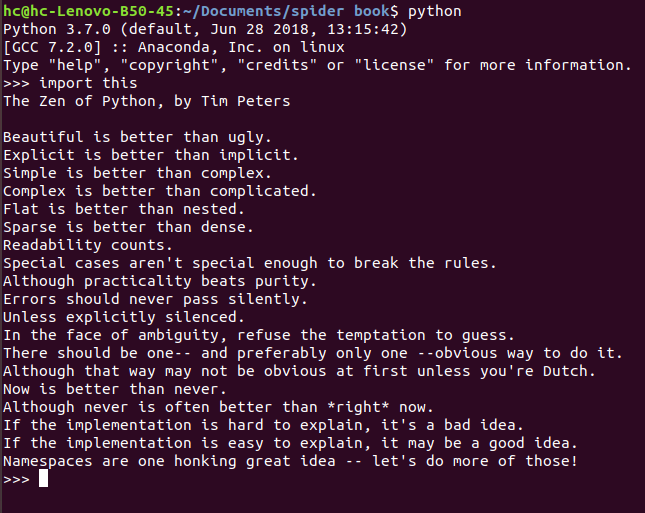
\includegraphics[width=\textwidth]{./figure/zen.png}
  \caption{Zen Of Python}
  \label{fig:zen}
\end{figure}

有点难懂对吧?我来“解释”一下吧。

\note{关于The zen of Python,网上有很多解释,仅供参考。一千个Pythoner就
  有一千零一个对The zen of Python解释,(还有一个是译文/原文),每个人,
  相同的人不同的时间,使用不同的Python版本,对The zen of Python 可能有
  不同的理
  解,\url{https://blog.csdn.net/gzlaiyonghao/article/details/2151918}
  这个博客里有译文。下面仅介绍其中几点个人理解。}

我一个很明显的特点就是代码美观,不像Java、C、C++等语言,通过丑陋的花括
号来规定作用域,我采用了\textbf{缩进}(\textbf{通常是4个空格})来规定作
用域的范围,因此看上去十分美观。

我的代码十分简洁明了,没有多余的分号。一般能用一句话实现功能的,就不会
用一个循环去实现(这样循环就多了,代码的层次、逻辑,就不再那么清晰)。
比如,我会用列表(集合、字典)表达式来代替循环。再比如,我有垃圾回收机
制,不用的东西,不用自行free\footnote{这方面博客很多,但是初学者不需要
  钻太深,只要知道有垃圾回收即可}。

\begin{python}
  # list comprehension l = [x**2 for x in range(1,10)]

  # print print(l)

  # for loop l=[] for x in range(1,10): l.append(x**2)

  # print print(l)
\end{python}

\code{2-1.py}

\note{这章里暂时不用完全理解代码的意思!但是如果你有精力,理解代码对你自
  己日后写Python代码也有好处}可以从\autoref{fig:2-1}看出代码的功能是一
样的,把所有的1-9的整数的平方的列表输出到控制台。另外,还可以看
出,Python虽然是一门面向对象的语言(如Java,c++),但是也支持面向过程
(如C)。因此,在编程的时候是很自由的。你不用编写主类,再编写一个主方法,
你甚至不用写一个主函数,只要你编写一段能被Python解释器(就
是\autoref{fig:2-1}中敲的python,类似于C里面的gcc和Java里的javac)“解
释”的代码,就能得到结果——或者正确,或者抛出异常。
\begin{figure}[htb]
  \centering 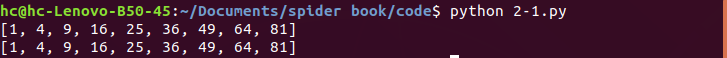
\includegraphics[width=\textwidth]{./figure/2-1.png}
  \caption{2-1.py运行结果}
  \label{fig:2-1}
\end{figure}

\note{在代码量大或者需要团队协作的时候,还是建议写上主函数,主函数怎么
  写优雅,会在下章讲述}

这里还要“解释”一下刚才为什么要反复特别强调“解释”这个词。和C、Java等编译
型语言不一样,我——Python不需要编译,而是由Python解释器,一步一步解释运
行。这样子,以牺牲少许性能为代价,节约了漫长的编译时间(如果你的电脑不
是很好,你又编译过大型的项目或者软件,你就知道编译有多么痛苦,Linux有些
发行版比如Gentoo等就是编译安装的,特别慢,编译一个gcc,要好几个小时。而
且编译语言,常常编译了好久没出错,到运行的时候再报错,然后又要debug,又
要再compile一次,很花时间),所以总得来说,我——Python,还是挺节约时间的。
另外,由于解释器的交互作用(输入一行Python代码,返回一个结果),我经常
被写这本书的家伙当作计算器用,无论是进制转换,还是快速幂,还是矩阵乘法,
抑或是简单的加减乘除,都有极其简单的调用方法,windows自带的calc里有的,
我都有,calc里没有的,我也基本都有,哪怕真的没有,我也可以造轮子般造出
来。

说完了我的主要优点,再说一下我的其它特点。

首先,我很慢,这主要归功于我是一门解释型的语言。也许有人不明白,为什
么“解释”就慢\footnote{关于Python慢的原因,感兴趣的同学可以参考这篇博客
  《为什么说python很慢》\url{https://www.jianshu.com/p/3fa56d9f58cb}。
  本书不会一一解释,仅挑选其中和语言特性有关的进行简单的讲解}。因为,一
个智能化的编译器可以预测并针对重复和不需要的操作进行优化。这也会提升程
序执行的速度。

第二,我很慢,因为我是动态性语言不是静态性语言,我在声明l是个list的时候,
不像java一样List<String> l = new ArrayList<String>()。而是l=[]。也就是
说,解释器在解释的时候,不知道l是什么类型,只知道l有没有定义过,只有在
运行的时候判断这个变量的类型,以及是否有对应的方法。具体
见\autoref{fig:type}。这个动态性的特点,让程序员在编程的时候可以少写很
多代码,但是如果程序员犯迷糊,就会帮倒忙(动态一时爽,调试火葬场),比
如字符串和整数(甚至小数)后面都可以接\%运算符,但是前者表示用数据来进
行格式化,代替\%d,\%s等占位符,后者是表示取模运算。\footnote{这点与c不
  同,主要体现在负数上,可以参考博
  客\url{https://blog.csdn.net/SharonLu1216/article/details/76774829}}
可以利用type类进行判断。

\begin{figure}[htb]
  \centering 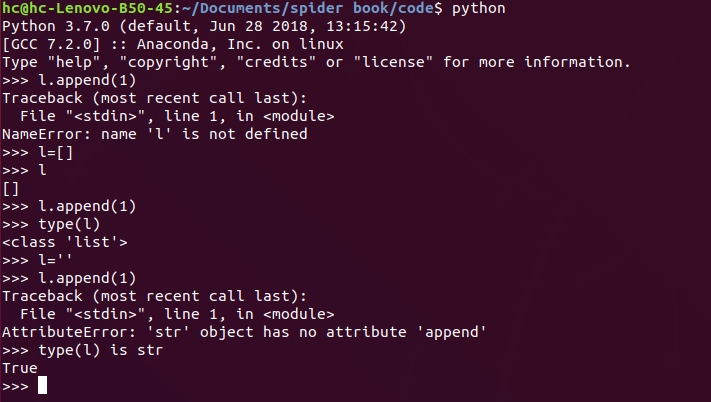
\includegraphics[width=\textwidth]{./figure/type.png}
  \caption{python动态类型}
  \label{fig:type}
\end{figure}

第三,我很慢,因为我支持多线程,但是支持得很不好,通俗地讲,叫鸡
肋,\footnote{关于Python为什么多线程鸡肋,推荐
  看\url{https://www.zhihu.com/question/23474039}里高赞的回答,虽然有点
  难}不能充分地利用cpu(开多个进程除外)。当然写爬虫嘛,没有太大影响,
因为爬虫主要是IO密集型的,计算量很少。所以我在进行CPU密集型的任务的时候,
会很慢。换句话来说,我不适合进行CPU密集型的任务。你可能要反驳我说:“深
度学习了解一下?”。那么,我要给你介绍一下我的绰号——“胶水语言”\footnote{关
  于胶水语言,可以参考知
  乎\url{https://www.zhihu.com/question/21626095}}。我一般来完成业务流
程,而需要性能的核心模块(比如numpy之类和科学计算有关的库)由我的兄
弟C/C++这样的语言来写。如果你快,那很OK,但是如果你不快还不会抱大腿,那
么非常Sorry,你是比不过我的。

Last but not the least,这回总算和慢不搭边了。我是强类型的语言!我是强
类型的语言!我是强类型的语言!重要的话说三遍!以后如果和别人介绍我,你
可以说我是动态类型的,但是如果你和别人说我是弱类型的,对不起,咱们不认
识!1+“1”=2,这叫弱类型(某一个变量被定义类型,该变量可以根据环境变化自
动进行转换,不需要经过显性强制转换。);1+“1”=报错,这叫强类型(如果不
经过强制转换,则它永远就是该数据类型了)。虽然稍微麻烦了一点,但是可以
避免很多Bug(Php:为什么每次躺枪的都是我)。

\aftercontent{本章介绍了一些Python的性质和特点,虽然内容有点枯燥,但是
  作者用幽默的语言(不要脸)进行了说明,对以后的学习会有点帮助。下章开
  始,要介绍Python的基本语法了。}


\chapter{Python语法基础}
\label{chap:programmar}

\beforecontent{Life is short, you need Python.}{Bruce Eckel}

\section{Python代码示例}
\label{sec:Python_code}

\note{本章开始,将广泛用到终端,Linux和windows都行,但笔者推荐Linux,因
  为后期用到docker,对一般人来说,Linux更方便,以下命令,如无特别指明,
  皆指Linux命令}

\begin{python}
  import requests req = requests.get('http://www.xicidaili.com/nn/')
  print('content',req.content,sep=': ') print(type(req.content))
  print('-'*10,'end','-'*10,end='来个换行吧')
\end{python}

\code{3-1.py}

\begin{figure}[htb]
  \centering 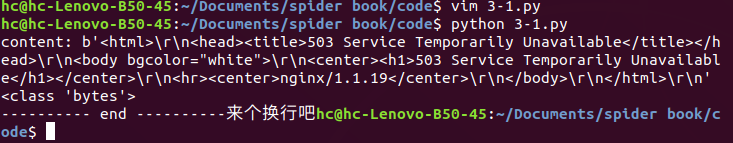
\includegraphics[width=\textwidth]{./figure/3-1.png}
  \caption{代码示例}
  \label{fig:3-1}
\end{figure}

结果如\autoref{fig:3-1}所示。

Excuse me?不是说好了这章讲语法的吗?一上来就扔了个代码和结果,让我们自
学?

非也非也!首先,我是要告诉你怎么运行python源代码(推荐命名为*.py)——python filename。如果你的目的是“系统地”学习语法,那么恭喜你,来错地方了。菜鸟教
程\footnote{Python3教程
  \url{http://www.runoob.com/python3/python3-basic-syntax.html}}和廖雪
峰的教程\footnote{Python教程 - 廖雪峰的官方网
  站
  \url{https://www.liaoxuefeng.com/wiki/0014316089557264a6b348958f449949df42a6d3a2e542c000}}
讲得比我更好,前者适合真菜鸟,后者适合假菜鸟(不会Python,但是其它语言
基础比较好),但是后者质量不错,比前者更好,能学到更多知识。

\note{个人觉得,直接讲语法,会有一些不懂的,或者因为厌倦而放弃,或者看
  似学会了,但不知道怎么用。给出代码,可以引起好奇心,哇,Python原来还
  有这种丧心病狂的功能!可以在给出的代码的基础上进行修改,写少量自己不
  会写的代码,避免重复劳动,做做实验,加深印象。}

接下来,我们打开终端(cmd),确保你已经配置好Python(包括pip)的环境变
量,以及requests库(Linux 用户可以通过pip list | grep requests命令来确
认是否安装requests库,或者输入python回车,import requests回车)。如果没有装requests库,在终端输入:pip install
requests;如果没有配置好环境变量,那么,请百度相关教程。

之后,输入Python,按照\autoref{fig:type_all},输入这些内容。
\begin{figure}[htb]
  \centering 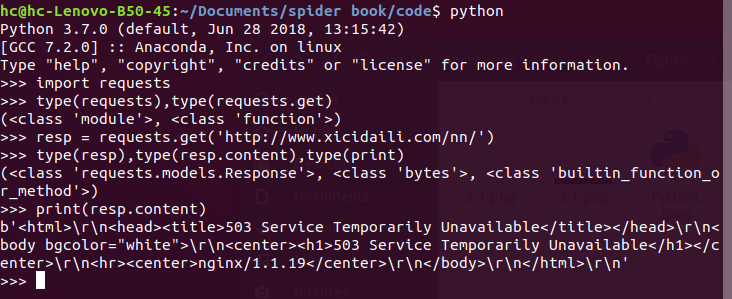
\includegraphics[width=\textwidth]{./figure/type_all.png}
  \caption{type所有变量}
  \label{fig:type_all}
\end{figure}

稍微总结一下,通过这些type,我们可以看到Python做了很多事:导入(import)
模块(requests)。调用模块(requests)里面的函
数(get)向\url{http://www.xicidaili.com/nn/}这个网站发送一个get请求,以
及调用Python内置的函数(print),将一个bytes类型的对象(响应的正文部分)输
出到控制台。然后还可以知道这些类名也好,函数名也罢,都是某个类的对象,
因此,一般的对象的操作(比如赋值)对函数名和类名等,都是可以使用的。也
就是说,我们在给自己的对象起名字的时候,\textbf{最好不要使用已经有的类
的名字,否则会覆盖原有的功能,除非你真的希望这样做。}

有了这些基础的认识,我们先来了解模块requests。

\section{模块}
\label{sec:module}

\tip{学习最好的方法就是模仿,尤其是有点基础的人,找个库的代码看看,可以
  学到不少知识。}

如\autoref{fig:find_requests}在终端中输入find 你的anaconda安装目录(我
是~/anaconda3) -name requests,然后,cd 进入其中一个文件夹。再执行ls命
令。

\begin{figure}[htb]
  \centering
  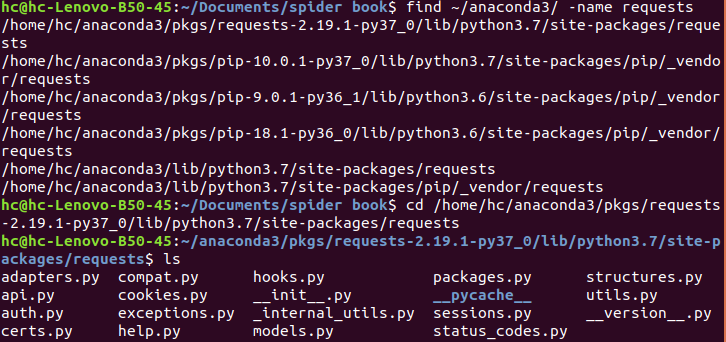
\includegraphics[width=\textwidth]{./figure/find_requests.png}
  \caption{寻找requests库的路径}
  \label{fig:find_requests}
\end{figure}

在这些文件中,有一个\_\_init\_\_.py,准确地说,每个Python的包里面都有一
个叫\_\_init\_\_.py的文件。\textbf{这是Python包和一般文件夹的本质区别,
  如果 \_\_init\_\_.py 不存在,这个目录就仅仅是一个目录,而不是一个包,
  它和里面的模块和嵌套包(比如numpy.linalg这个numpy包的子包)就不能被导
  入。}因此,我们如果有自己写一个包的时候,千万不要把\_\_init\_\_.py的
文件给删除了,宁可放一个空的\_\_init\_\_.py的文件(IDE一般会自动为我们
创建一个\_\_init\_\_.py,不用我们自行创建)。

接下来,我们可以看一下requests包的\_\_init\_\_.py文件,看一下怎么编
写\_\_init\_\_.py文件,以及涉及的一些Python语法。

用编辑器
(Linux下的gedit,vim/vi,emacs,nano等,windows下的notepad++,notepad等
或者一些跨平台的如sublime text)打开\_\_init\_\_.py文件,或者
用spider,Pycharm的IDE的代码跳转等功能,或者去github或pypi上搜
索requests\footnote{这种方法不一定能找到所有的库。requests github:
  \url{https://github.com/requests/requests/blob/master/requests/__init__.py}
  pypi: \url{https://pypi.org/project/requests/}}查看\_\_init\_\_.py的
代码。

\note{PyPI(Python Package Index)是python官方的第三方库的仓库,所有人都
  可以下载第三方库或上传自己开发的库到PyPI。PyPI推荐使用pip包管理器来下
  载第三方库。}

100多行的代码,看下它做了怎样的事。(版本不同,代码可能有一些不同)。

第一行,\# -*- coding: utf-8 -*-声明编码方式为utf-8。

第3-6行,\#开头,用于注释,会被解释器读取(如声明编码),但不会被执行。
这里画了一个Requests。(丑)

后面许多行被2对3个双引号包括,表示多行字符串,关于字符串,
在\autoref{sec:string}节会讲述。讲述了requests库的基本用法。

第43行到46行导入了一些模块。到这里,已经出现了两种导入模块的方法。那么
这里就总结一下,顺便剧透一下剩下的用法,以requests库举例。

\begin{enumerate}[1)]
\item import 模块。调用:该模块.对象(如果是这里的对象是广义的对象,通
  过这段时间的学习,相信你已经能够意识到,模块名,函数名,类名,变量,
  这些其实都是一个对象的引用)举例:import requests然后r =
  requests.get('http://www.baidu.com')
\item from 模块 import 对象。调用:该对象。举例:from requests import
  get然后get('http://www.baidu.com')
\item import 模块 as 别名。调用:别名.对象,不能用该模块名.对象访问。
  (模块名比较丑的时候,比较好用)import numpy as
  np 然后a=np.mat([[1,2],[1,3]])
\item 模块可以用相对路径引用,.模块,..模块,见46行,*可以匹配所有对
  象。
\end{enumerate}

\tip{如果你感到没有看懂,可以在Python解释器中输入globals()函数,用各种
  方式导入一个模块,再输入globals()函数,看看有什么区别,你就明白了}

接下来是2个def代码,我们暂时先不要仔细地看下面的内容,只要知道这是2个函
数,里面用了if控制流程即可。后面是捕获异常。后面就没啥熟悉的知识了。

代码的结构已经剖析完了,接下来来聊聊为什么要用模块。

我们写模块的目的是,让代码模块化,更容易复用。在这方面做得比较好的,除
了模块,还有俩,一个是函数,一个是类,而且,在模块中,函数和类也是很常
见的,或者是写在模块本身,或者是写在其它模块被导入。

\subsection{函数}
\label{sec:function}
函数,在c里面见过,但是,如果只是C里函数的功能,那么这门语言就不配用“人
生苦短,我用Python”这句广告了。Python中的函数究竟有什么强大之处?

首先,由于Python是动态类型的,所以不用声明返回类型,参数也不用类型。

第二,由于Python内置的数据结构元组(tuple)(见\autoref{sec:tuple}),
使得\textbf{Python可以返回0-多个返回值。}

第三,Python可以给函数提供默认参数,默认参数的存在,使得Python函数的调
用,千变万化,可以省略默认参数,可以提供不同功能(在函数中加上if),类
似于Java中的方法重载,却比它简单得多。不过,无论是函数,还是方
法,Python都不支持重载,因为,函数名或者方法名,本身就是一个对象的引用,
如果你定义了两个相同名字的对象,那么后面一个势必会取代前面一个,把它覆
盖,你将无法调用前面一个。另外需要注意,有默认值的参数,必须放在无默认
值的参数后面。

第四,Python在调用函数写实参的时候,可以为每个参数添加函数名来增加可读
性,也方便程序员编码,因为由于你指定了名字,Python解释器就可以机智地区
分他们,可以少记很多参数的顺序,
如requests.get(headers=\{\},url='http://www.baidu.com')(我们可以把它叫
做关键字参数,调用实参的时候没有函数名的参数叫位置参数)。关键字参数必
须放在位置参数的后面。

\tip{关于关键字参数必须放在位置参数的后面这一点,可以参考数学中的排列组
  合问题——排队,有位置限制的,必须先排,没位置限制的,可以放到他们排好
  以后再排,在Python中,位置参数就是位置有要求的参数}

\note{Python中的函数和方法没有访问权限这一概念,如果你不希望你的方法被
  其它模块调用,请以\_开头命名函数}

\note{对于简短的函数,可用lambda表达式代替,f1=lambda :'hello
  world',f2=lambda x,y:print(x+2*y)}

\subsection{类}
\label{sec:class}

和类联系在一起的一个概念,就是面向对象,由于爬虫涉及的面向对象的知识很
少,这里就作一个简单的介绍,如有需要,可以查找网上的教程。

类,用class 类名(父类名):声明。一个类里面存在0个或多个方法。方法,可
以理解成和类绑定在一起的函数,但是比函数多了一个self参数,表示函数所属
的对象本身。其中有一些魔法方法,开头和结尾都有2个\_,\textbf{在特定的时
  期会调用}。比如\_\_init\_\_,在类初始化的时候调用,可以理解成java中类
的构造方法,还有一些魔法方法,实现它们可以让我们以更简单的方法去调用它
们,后面要讲的列表,字典,之所以调用如此方便,就是因为在编写这些类的时
候,实现了其中的一些魔法方法。函数或方法,之所以对那么多种类的对象都适
用,因为某些函数在编写的时候,并不是直接处理对象的,而是,\textbf{调用
  对象写好的魔法方法},对于魔法方法,我们不需要过多关心,了解它们存在即
可。

创建类,用类名(参数)的方式,比如a=list((1,2,3))

另外,Python没有接口的概念,Python有多重继承,但是不常用,继承其它类,
一个父类基本够用,调用父类的方法用得不多,可以用到时百度。

\section{常用内置数据结构}
\label{sec:data_structrue}
Python好用的一个原因,就是内置了许多好用又常用的数据结构,比如字符串,列
表,元组,字典等,每种数据结构都有很多丰富的好用的方法。

\subsection{字符串}
\label{sec:string}

字符串(比如'Python',"py")用一对单引号或一对双引号表示,基本没有区别,
在引号内有双引号时,推荐用单引号,在引号内有单引号时,推荐用双引号,否
则需要转义。

多行字符串用一对3引号表示,用于注释或说明。

字符串里,有很多常用的方法。如\autoref{fig:string}所示。这个内置数据结
构将在以后频繁用到。

\begin{figure}[htb]
  \centering 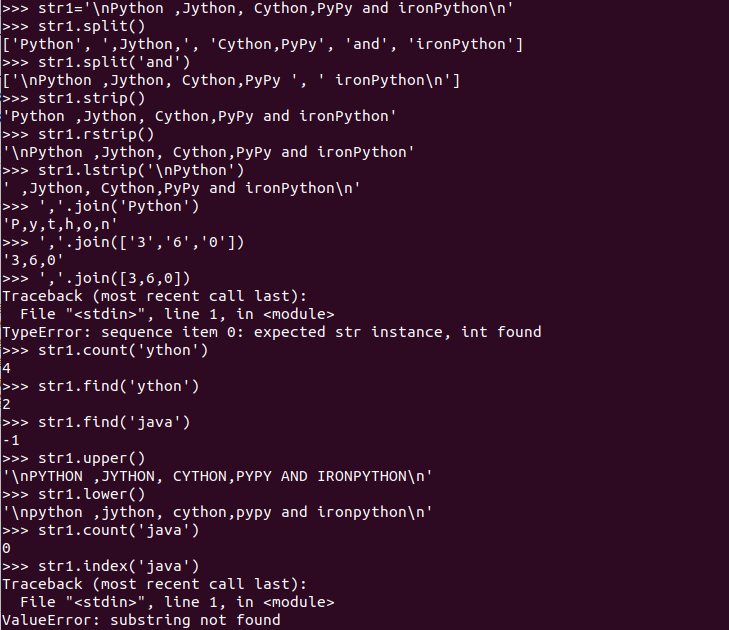
\includegraphics[width=\textwidth]{./figure/string.png}
  \caption{Python}
  \label{fig:string}
\end{figure}

strip默认去除字符串两侧的中英文空格,制表符 \verb|\|t,换行
符 \verb|\|r, \verb|\|n等,添加参数,可以使指定字符去掉。l表示left,r表
示right。

split方法指定分隔符对字符串进行分割,甚至还可以指定次数,默认全部分割。

string模块的函数\textbf{不支持正则表达式},如果想调用正则表达式,请
用re模块。

join用指定参数将参数们连接到一起(参数必须可迭代的字符序列,比如字符列
表,字符元组,字符串等)

replace方法返回替换后的对象,但不对参数本身进行修改。

find和index方法可以检测字符串中是否包含子字符串 str ,如果指定 beg(开
始) 和 end(结束) 范围,则检查是否包含在指定范围内,如果包含子字符串
返回开始的索引值,否则find返回-1,index抛出异常。

count方法返回字符出现的次数。

字符串中的$\backslash$表示转义字符,如果在正则表达式或者路径中,需要用
到,要用2个$\backslash$来代替。或者用r'$\backslash$ is a backslash'的方
式(外面加个r表示raw,里面的$\backslash$不转义)。

\subsection{字节}
\label{sec:bytes}

字节(bytes)既不好用,又不常用,但是在爬虫中又偏偏要用到。

字节用b''表示。
如b'<html><body></body></html>'。这里要掌握它与字符串的互相转换。

字符串转字节,用''.encode()方法。字节转字符串用''.decode()方法。可以添
加参数,一般为'UTF-8'

\subsection{列表}
\label{sec:list}

这是一类十分常用的,像数组,链表的东西。但是,列表里,可以是任意类型的,
可以是任意长度的。

\begin{figure}[htb]
  \centering 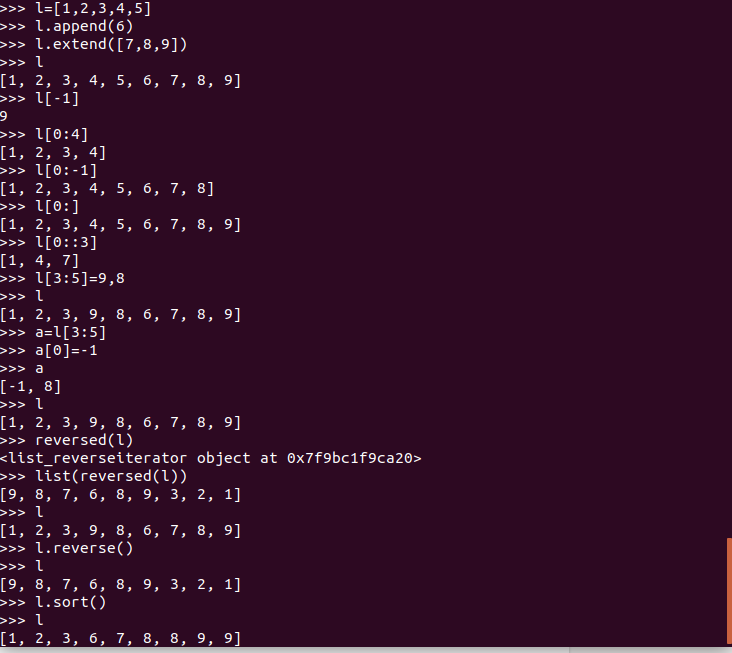
\includegraphics[width=\textwidth]{./figure/list.png}
  \caption{list}
  \label{fig:list}
\end{figure}

列表用[]表示,类名list。

append方法在后面添加指定对象,extend在后面用参数列表延展原列表。

Python列表索引从0开始,支持负索引,即右往左数。

切片是Python又一丧心病狂的语法糖。格式为l[start:end:step]支持正向切、反
向切、跳着切、切到底、切一半、边切边改、切了当拷贝。包括start但不包
括end。

\note{关于切片什么时候会改变原值,什么时候不会,请自行思考(考虑一下引
  用)并实验}

切片的强大,使得一些list的方法不常用了,比如reverse方法和内置
的reversed函数。

\note{Python里有很多像reverse,reversed这样命名的方法或函数,比
  如sort,sorted,性质有所不同。前者改变自身,后者不改变自身,而是返回一
  个拷贝。}

\tip{时间久了可能会记反,这里给出一个我的记忆方式,英语中,动词+ed,是
  过去分词,常常用来当形容词。因此,sorted函数返回一个形容词版(有序的)
  的列表,不改变列表本身。而sort是方法,表示一个对象的行为或者动作,这
  个行为或动作的对象是self,即列表本身。}

\note{reversed方法返回一个生成器,sorted方法返回一个列表。生成器可以生
  成列表,但是不会立即生成,在用for语句迭代的时候和列表相似,所以比较节
  约内存。}

\subsection{元组}
\label{sec:tuple}

元组用(1,)或(1,2,3)表示,()可以省略(如果不会发生歧义,比如交换变量,可
以省略(),但是函数参数那里,就不能省略)

元组和列表十分相似,所以,不介绍它的语法了。唯一的区别是,元组不支持修
改。类名为tuple。

元组可以干啥?函数多值返回,并行赋值(交换两个变量可以用a,b=b,a),可以
当字典的键(这点列表不行)。

\subsection{字典}
\label{sec:dict}

字典是Python中又一好用的数据结构,类名dict,用{key1:value,key2:value}表示,
特点是可以直接根据键名获取键值。一方面,用过其它语言map数据结构的人,都
知道map有多好用,存取有多方便。另一方面,现在很多网页都是通过json格式传
输数据的,这意味着爬虫有时需要抓取json格式的数据。而json和字典一样,都
是键值对的形式,这意味着,json和dict可以方便地转换(标准库里
的json.dumps,json.loads,json.load,json.dump)。有些NoSQL(比如Mongodb)
也是键值对类型的,因此,也可以通过dict来封装对应的数据。

\tip{这里,又出现了令人混淆的函数名,可以这样记忆dumps,loads的s可以记忆
  为string,说明这两个函数是对string类型操作,剩下两个是对文件操作。}

dict的基本用法可以见\autoref{fig:dict}。

\begin{figure}[htb]
  \centering 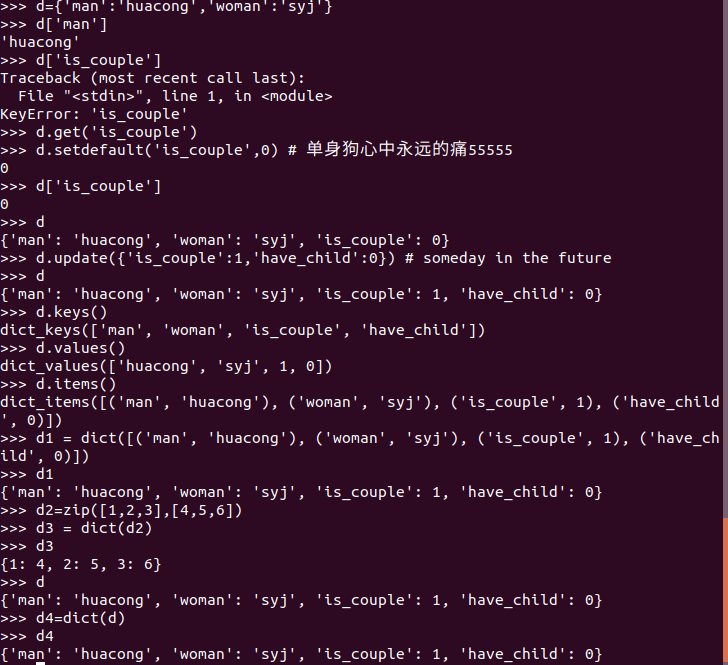
\includegraphics[width=\textwidth]{./figure/dict.png}
  \caption{dict用法}
  \label{fig:dict}
\end{figure}

假设字典的名字叫d。

获取键值的方式有3种,一种是d[键名],一种是d.get(键名),一种
是d.setdefault(键名,默认值)。区别在于,在不存在键名的时候,用d[键名]获
取键值会报错,get方法会返回None(类似于c里的NULL各java里的null,以及一
些其它语言中的nil)。d.setdefault方法会返回默认值并修改字典。

update允许用新的字典去更新旧的字典。如果旧字典没有对应的键,那么旧字典
会增加对应的键名和键值。如果旧字典有对应的键名,那么新字典会更新对应的
键值。如果新字典没有对应的键名,那么旧字典对应的键值不会被改变。

d.keys()方法获取字典的键名的集合(dict\_keys)。之所以叫作集合,因
为,\textbf{字典里不会有相同的键值}。键名必须是不能修改的对象,比如元组,
字符串,数字,但不能是可以修改的对象。

d.values()方法获取字典里的键值列表(dict\_values)。

d.items()方法获取字典里的键值对的列表(dict\_items)。

zip可以但不仅限于将用作键名的列表,和用作键值的列表,打包成键值对元组的
列表(可以是任意的列表)。

\subsection{集合}
\label{sec:set}

集合用得不多,但是可以看看\autoref{fig:set}。

\begin{figure}[htb]
  \centering 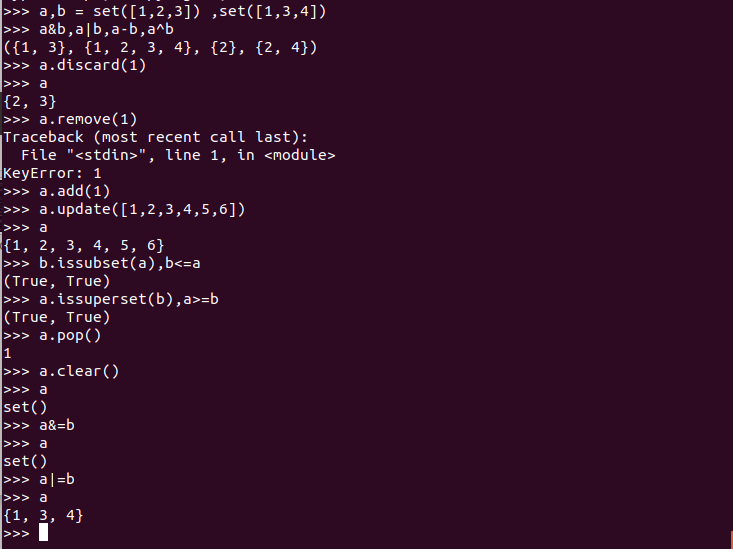
\includegraphics[width=\textwidth]{./figure/set.png}
  \caption{set用法}
  \label{fig:set}
\end{figure}

数学里的集合是无序的,不重复的,Python亦然。对于集合,Python支持用操作
符和方法来完成。现用一张表格来总结,其中
\begin{align*}
  A=\{1,2,3\}\\
  B=\{1,3,4\}
\end{align*}


\begin{table}[htb]
  \centering
  \caption{Set用法}
  \begin{tabular}[htb]{|p{5cm}|l|l|l|}
    \hline
    操作&结果&操作符&方法\\
    \hline
    并集& $\{1,2,3,4\}$&a|b & a.union(b)\\
    \hline
    交集& $\{1,3\}$&a\&b & a.intersection(b) \\
    \hline
    差集& $\{2\}$&a-b & a.difference(b) \\
    \hline
    相对差集& $\{2,4\}$& a$\land$b & a.symmetric\_difference(b) \\
    \hline
    A真包含于B& False &a<b & a.issuperset(b) \\
    \hline
    让set “A”只保留set “B”中有的元素&None &a\&=b & a.intersection\_update(b) \\
    \hline
    让set “A”添加set “B”中有的元素&None &a|=b & a.update(b) \\
    \hline
    让set “A”变成AB的相对差集&None &a$\land$=b & a.symmetric\_difference\_update(b) \\
    \hline
    让set “A”变成AB的差集&None &a-=b & a.difference\_update(b) \\
    \hline
  \end{tabular}

  \label{tab:usage_of_set}
\end{table}

remove方法和discard方法,都可以去掉集合中的元素,区别在于当集合中没有指
定元素的时候,前者抛出异常,后者什么都不执行。

clear方法可以清除所有的元素。

\section{流程控制}
\label{sec:control}

\subsection{选择}
\label{sec:choose}
\begin{python}
  if 情况1:# 情况不用加括号
      做一些事
  elif 情况2:# 可选 else if的意思
      pass #啥都不做,相当于java和c中的;
  elif 情况3:
      做另外的事
  else:# 可选
      啥都不做
\end{python}
\code{if-elif-else}

\note{Python中没有switch-case语句,因为switch-case和if-elif-else代码量
  差不多,功能也一致,the zen of Python里有一条There should be one--
  and preferably only one --obvious way to do it.}

Python条件,用and,or,not来连接,不用\&\&,||,!。

Python允许2<money<=3这样的写法。

is 判断是否是同一个对象(id(对象)是否相等),==判断值是否相等。

c/Java中的a?b:c的条件表达式,在Python中写作b if a else c。返回b(如果满足条件a的话)否则返回c。

\subsection{循环}
\label{sec:loop}

\subsubsection{for}
\label{sec:for_loop}
\begin{python}
  for 变量 in 可迭代的对象:#可以是列表,元组,字典,集合,range对象、生成器等
      做一些事
  else: # 可选,当for循环中没有成功break时
      做别的事
\end{python}
\code{for-else}


\subsubsection{while}
\label{sec:while_loop}

\begin{python}
  i=0
  while 条件成立:
      i+=1 # 没有i++的说法
  else:
      做别的事
\end{python}

\code{while-else}

\subsection{异常处理}
\label{sec:exception}

\begin{python}
  try:
      raise Excepption('some string')
  except KeyError as e:# 捕捉到异常1并垂命名
      pass
  except (NameError,TypeError):# 捕捉到2种异常,按相同方式处理
      pass
  except:
      pass
  else:
      pass
  finally:# 无论如何都会进行,用于关闭数据库连接等。
      pass
\end{python}
\code{try-raise-except-finally}
\section{其它特性}
\label{sec:other_features}

嵌套。由于Python是动态类型,因此,你可以很容易地构建出多维列表等高级的
数据结构。

关键字in可以检查对象是否在(列表,元组,字符串,字节,字典的键名,集合
中)。

del语句可以按照索引删除列表元素、按照键名删除字典元素。

assert用于断言。

*可用于重复,比如'python'*10。

+可用于字符串、元组、列表的拼接。

\%可用于字符串格式化和求模(c、java、c++中是求余)。

Python支持按位与、按位或、按位非、移位运算。

int,float,str,list,tuple,dict等都可以用对应的类名进行转化。

yield 类似return ,不同点在于yield返回值后还会继续进行,使用了 yield 的函数被称为生成器,用next函数调用,得到下一个值。生成器的好处是只有在调用的时候才会生成相应的数据(调用到这个数据的时候才会生成这个数据,没有调用到时就没有这个数据),只记录数据的当前位置。

可以用列表/集合/字典/元组表达式配合条件表达式等完成列表/集合/字典/生成器的初始化。

\begin{python}
  a = [[1 if i==j else 0 for i in range(3)] for j in range(3)]# 三阶对角阵
  b = {x**2 for x in range(-5,5)}# {0,1,4,9,16,25}
  c = (x for x in range(3))# 生成器
\end{python}
\code{list comprehension}

在一些函数中的定义中,还可以看到,函数的参数还有*args,**kwargs,分别用于多个位置参数,和多个关键字参数,实际上用到的数据结构为元组和字典。

在调用的时候也可以用*[],**kwargs,不常用,在参数较多的时候用。

\begin{python}
def a(*x):
    print(x)

def b(**y):
    print(y['a'],y)

def c(a,b,c,d):
    print(a,b,c,d)

def d(a,b,c=1,d=2,e=5,f=6):
    print(a,b,c,d,e,f)

a([1,2,3,4,5])# 调用的时候只有一个位置参数。
b(**{'a':1,'b':2,'c':3,'d':4})# 不加星相当于1个位置参数。
c(*[1,2,3,4])# 调用的时候,相当于4个位置参数。
d(*[1,2,3],**{'d':3,'e':4,'f':5})# 调用的时候,3个位置参数和3个关键字参数。
\end{python}
\code{args-kwargs}

到现在Python的基本语法已经讲得差不多了,还有文件读写和面向对象没讲,留到需要用到的时候再拓展。可以再看看requests,或者找一些标准库的模块,是不是好懂很多(当然有些函数不是用Python实现的,所以你可能找不到Python代码)。

学完了这么多,稍微放松一下。

\begin{python}
import sys
寻找女朋友=lambda x:print('%d岁,寻找女朋友ing...'%x)
结婚=lambda x:print('%d岁,结婚啦,xswl'%x)
单身=lambda :print('emmm其实单身也挺好...')
等死=lambda:print('等死,人最终还是要死的,也不知我死的时候是一个人还是两个人,都有可能')

def 生活(结婚年龄):
    for 年龄 in range(5):
        print('%d岁,没印象,应该单身吧?'%年龄)
    for 年龄 in range(5,10):
        print('%d岁~%d岁,有印象,单身!'%(年龄,年龄+1))
    for 年龄 in range(10,20,2):
        print('%d岁~%d岁,依然单身'%(年龄,年龄+2))
    while 40>年龄 >=18:
        try:
            寻找女朋友(年龄)
            还没找到女朋友 = 年龄<结婚年龄-3
            if 还没找到女朋友 and 年龄<30:
                continue
            elif not 还没找到女朋友:
                pass
            else:
                raise Exception('唉,注孤生')
        except Exception as e:
            print(e)
        else:
            结婚(年龄+3)
            return
        finally:
            等死()
            年龄+=1
    单身()

if __name__=='__main__':
    assert len(sys.argv)==2,'输入结婚年龄哦'
    结婚年龄=int(sys.argv[1])

\end{python}

\aftercontent{本章介绍了Python的基本语法,内容较多,但较为枯燥,但是这些内容是后面内容的基础。下章开始介绍爬虫。}

\chapter{爬虫基础}
\label{chap:spider_foundation}

\end{document}
